\section{Hardware}\label{sec:hw}
\subsection{Diagrama en bloques general}
El sistema se compone de módulos funcionales que interactúan entre sí, estos son: el \emph{maestro}, el cual recibe los datos recibidos y los \emph{esclavos} que actualizan una matriz, en la figura \ref{fig:diagrama-bloques-general} se puede observar el diagrama en bloques de todo el sistema.

\begin{figure}[!ht]
	\centering
	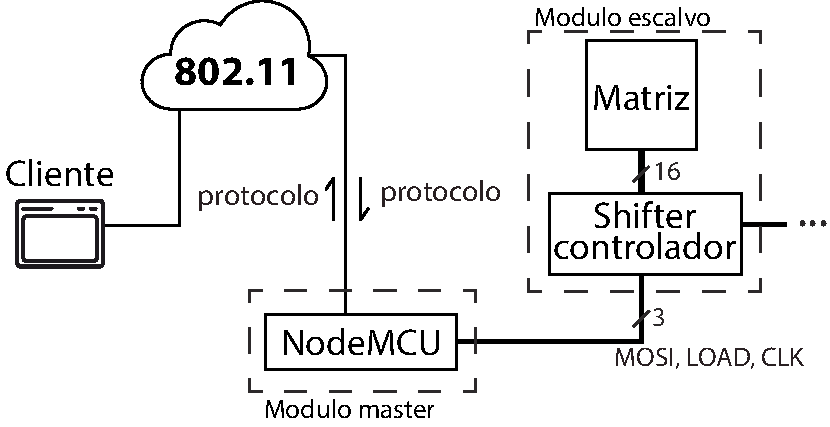
\includegraphics[width=\linewidth]{imagenes/hw/diagrama-bloques-general.pdf}
	\caption{Esquema general entre todos los componentes del sistema.}
	\label{fig:diagrama-bloques-general}
\end{figure}

\subsection{Fuente de alimentación}
El sistema recibe una fuente alimentación de forma externa, la cual es de 5V para abastecer los componentes internos. Para ello, de decidió incorporar un Jack (de 5.5mm x 2.1mm) a modo de interfaz.

\subsection{Módulo maestro}
Como se mencionó anteriormente, este modulo se encarga de procesar los datos enviados desde el cliente y controlar los demás módulos.

Su componente principal es el microcontrolador NodeMCU, que integra un AI-Thinker ESP-12E (figura \ref{fig:foto-esp12e}), el cual contiene un SoC (\emph{System on Chip}) ESP8266EX (figura \ref{fig:esp8266ex}) de la empresa Espressif. El módulo NodeMCU es hardware libre, sin embargo, el ESP12E y el ESP8266EX no lo son.\cite{NodeMCU}

\begin{figure}[ht!]
	\begin{center}
		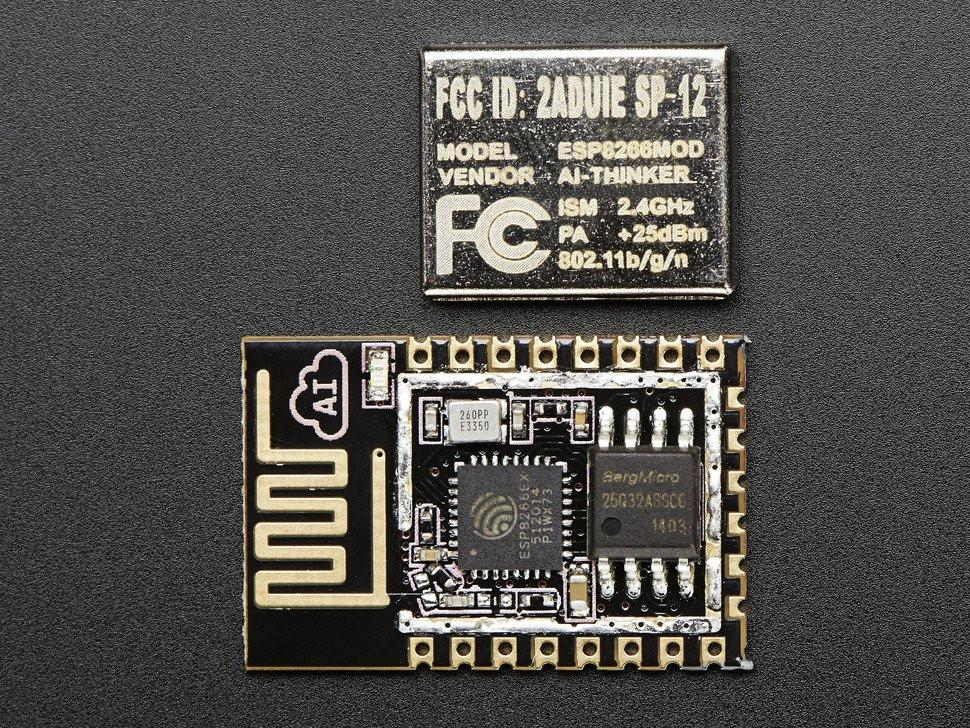
\includegraphics[width=8cm]{imagenes/esp12e-foto.jpg}
		\caption{Foto del módulo ESP12E sin su cubrimiento.}
		\label{fig:foto-esp12e}
	\end{center}
\end{figure}

\begin{figure}[ht!]
	\begin{center}
		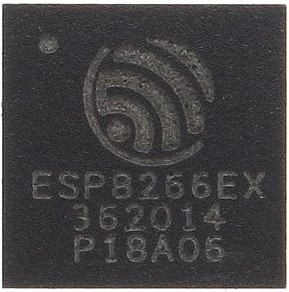
\includegraphics[width=3cm]{imagenes/esp8266ex.jpg}
		\caption{Foto del integrado ESP8266EX.}
		\label{fig:esp8266ex}
	\end{center}
\end{figure}

\begin{figure}[ht!]
	\begin{center}
		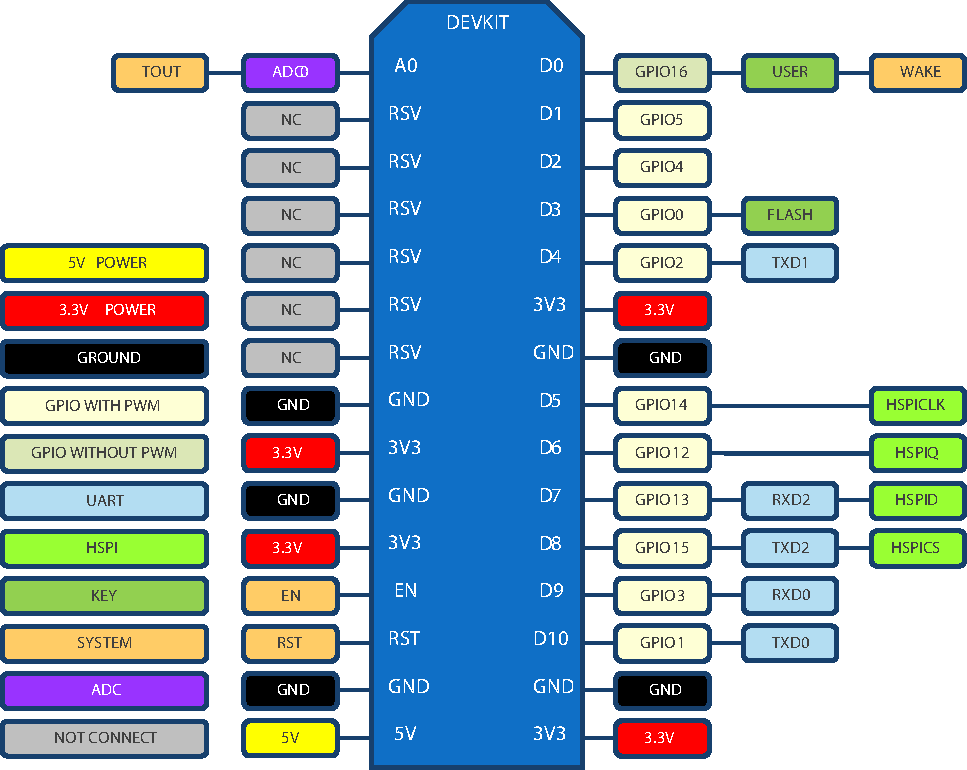
\includegraphics[width=0.95\textwidth]{imagenes/nodemcu-pinout.pdf}
		\caption{Asignación de pines del NodeMCU.}
		\label{fig:nodemcu-pinout}
	\end{center}
\end{figure}

Es importante tener en cuenta que el sistema no integra en su hardware directamente ni el ESP12E ni el ESP8266EX, sino que integra el NodeMCU, cuya asignación de pines se puede ver en la figura \ref{fig:nodemcu-pinout}.

El chip ESP8266EX combina un microcontrolador Tensillica Xtensa L106, un RISC de 32 bits corriendo a 80 Mhz, con funcionalidad WiFi. \cite{ESP8266Datasheet} El chip tiene memoria ROM con firmware no removible, y puede correr programas almacenados en flash externa. Para poder usar todas sus funcionalidades, se debe programar sobre firmware privativo desarrollado por Espressif, esto implica que el programa de usuario corre en simultáneo con el firmware y el uso de la memoria de trabajo está sujeto a la versión del firmware. Según el datasheet, el usuario puede esperar tener disponible 50 KiB de SRAM.

Como se mencionó anteriormente, se necesita de flash externa para correr programas. El módulo ESP-12S se encarga de proveer al ESP8266EX 4 MiB de memoria flash.

\subsection{Módulo esclavo}
Un modulo esclavo posee un driver MAX7219, que es el componente principal junto con una interfaz que permite conectarse a otro módulo esclavo o en su defecto al master.

\subsubsection{MAX7219}
El MAX7219 es un controlador compacto, de entrada y salida en serie de cátodo común que conectan microprocesadores a LEDs numéricos de siete segmentos de hasta ocho dígitos, pantallas de gráfico de barras o 64 LED individuales. Se incluyen en el chip, un decodificador BCD, circuitos de multiplexación, controladores de segmentos y dígitos, y una RAM estática de 8x8 que almacena cada número. Solo se necesita una resistencia externa para configurar la corriente de segmento para todos los LEDs.

El MAX7219 es compatible con los protocolos SPI, QSPI y Microwire, y tiene controladores de segmento de velocidad limitada para reducir el EMI.

Los dígitos individuales se pueden actualizar sin reescribir toda la pantalla. El MAX7219 también permite al usuario seleccionar el código de decodificación o no decodificación para cada dígito.

Su alimentación V\texttt{+} debe estar entre 4 y 5.5 Volts para su correcto funcionamiento. En cambio los voltaje de las entradas lógicas tienen una restricción de que un valor alto como mínimo debe ser 3.5V y un valor bajo como máximo 0.8V.

Las características principales que posee el chip integrado se enumeran a continuación:
\begin{itemize}
	\item Interfaz serie de 10 MHz.
	\item Control de segmento LED individual.
	\item Selección de dígitos Decode / No-Decode.
	\item Apagado de baja potencia de 150 microA (datos retenidos).
	\item Control de brillo digital y analógico.
	\item Pantalla borrada al encenderse.
	\item Unidad de visualización LED de cátodo común.
	\item SPI, QSPI, interfaz serie Microwire paquetes DIP y SO de 24 pines.
\end{itemize}

La disposición de los pines del MAX7219 se puede observar en la figura \ref{fig:MAX-pines} y la descripción de cada uno en la tabla \ref{table:MAX-pines}.

Es necesario prestar atención en el conexionado con respecto a los pines de tierra (GND) ya que ambos deben estar conectados para el driver pueda funcionar correctamente, ambas estan al lado izquierdo de la figura \ref{fig:MAX-pines} (Pin 4 y 9).

Por otro lado, el MAX7219 tiene un pin denominado DOUT (pin 24) se utiliza para encadenar varios MAX7219 y de esta forma pasar la información al que esta directamente conectado, éste pin nunca tiene alta impedancia.

\begin{figure}[htp!]
	\centering
	\begin{center}
	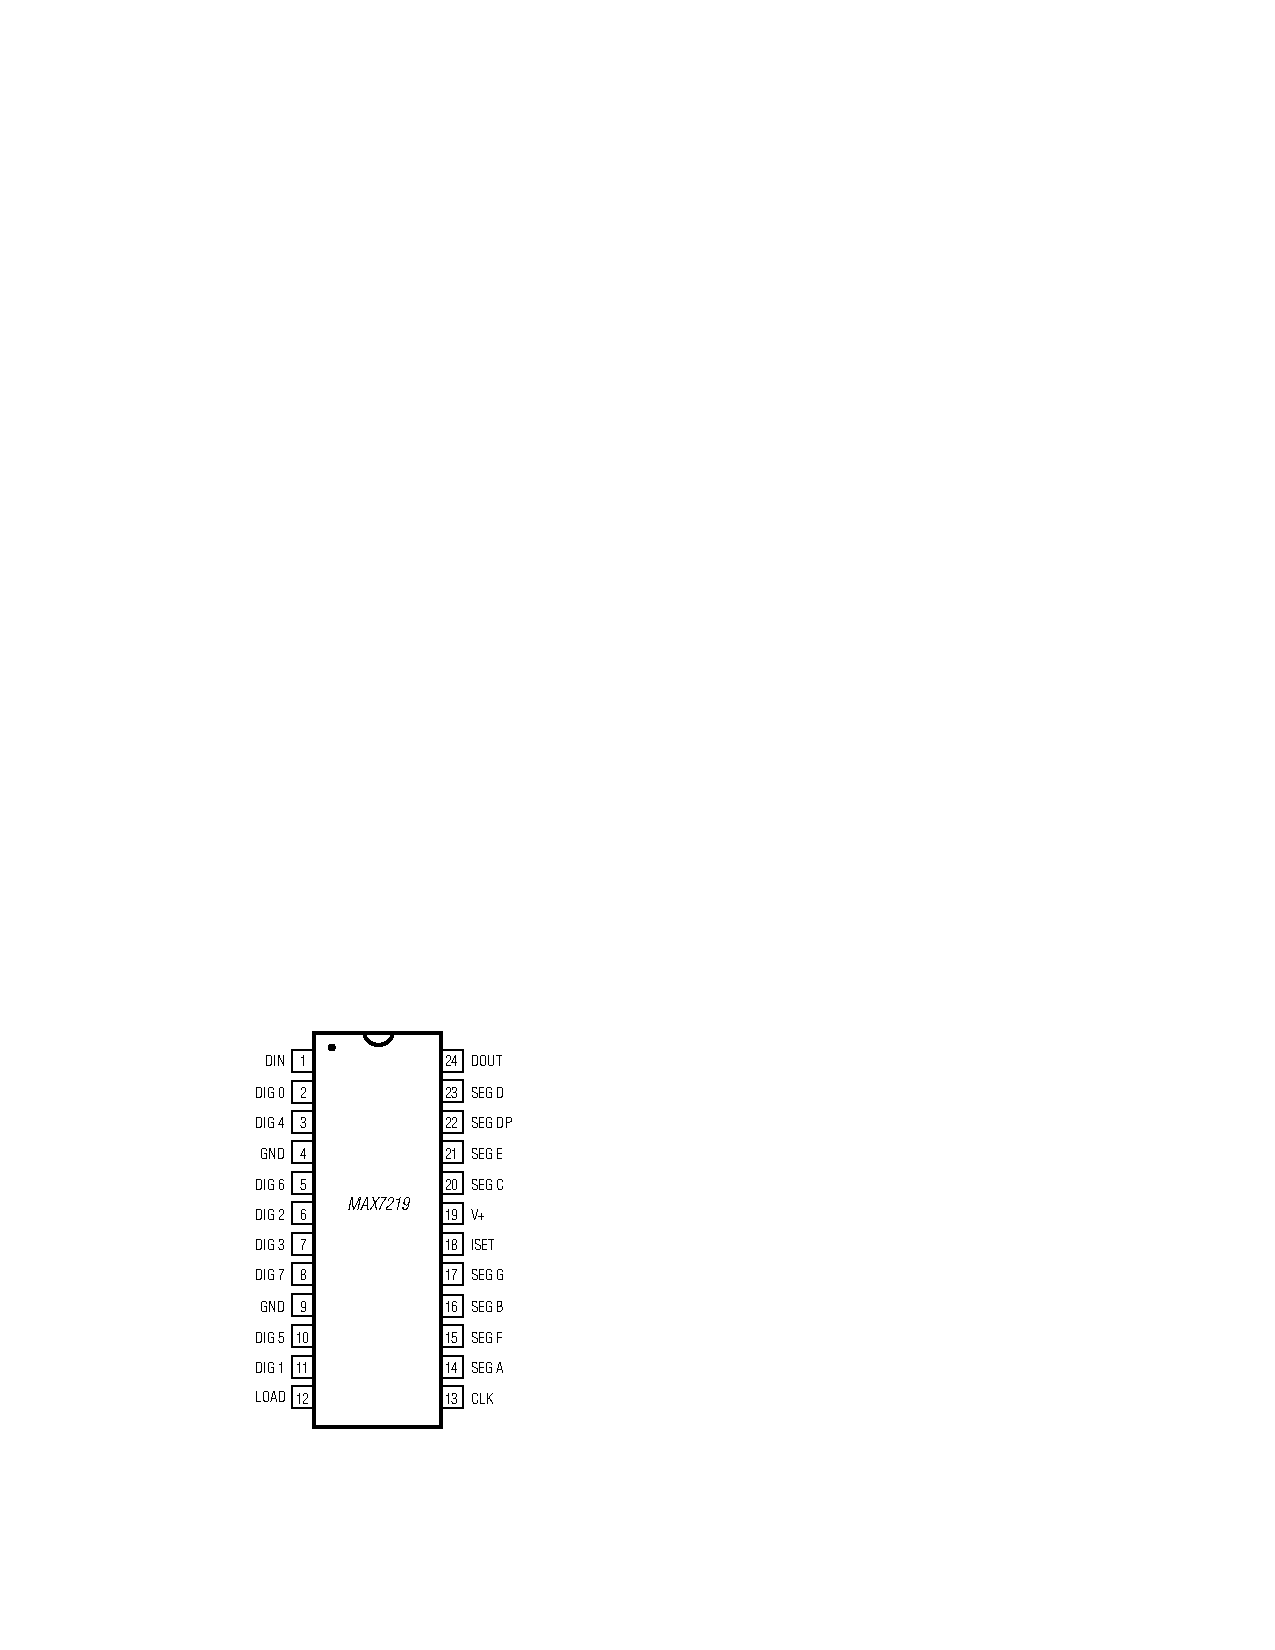
\includegraphics[scale=1.2]{imagenes/hw/max.pdf}
	 \caption{Configuración de pines del chip MAX7219.}
	  \label{fig:MAX-pines}
	\end{center}
\end{figure}

\begin{table}[htp!]
\centering
\caption{Descripción de los pines del MAX7219}
\label{table:MAX-pines}
\begin{tabular}{C{10mm} C{14mm} L{108mm}}
\hline
Pin               & Nombre          & Función    \\ \hline
1                 & DIN             & Pin de datos seriales. Los datos son cargados en el registro de 16 bits en cada flanco ascendente del clock. \\
2, 3, 5–8, 10, 11 & DIG 0 - DIG 7    & Líneas de transmisión de ocho dígitos que absorben corriente del cátodo común de la pantalla. El MAX7219 deja en V+ cuando esta apagado. Los dígitos están en alta impedancia cunado se apaga.\\
4, 9              & GND             & Tierra.\\
12                & LOAD            & Pin de control. Los últimos 16 bits del Serial Data son cargados en el flanco ascendente. \\
13                & CLK             & Pin de clock serial. En cada flanco ascendente, los datos sin shifteados dentro de un registro interno. En cada flanco descendente los datos salen de DOUT. En el MAX7221, la entrada CLK está activa solo mientras LOAD está baja. \\
14–17, 20-23      & SEG A–SEG G, DP & Las unidades de siete segmentos y el punto decimal impulsan la fuente de corriente a la pantalla. Cuando un controlador de segmento está apagado, se conecta a GND.\\
18                & ISET            & Conectar a  $V_{DD}$ a través de una resistencia ($R_{SET}$) para configurar la corriente que pueda entregar a los dígitos y segmentos. \\
19                & V+              & Fuente positiva de corriente, conectar a 5 V. \\
24                & DOUT            & Salida de datos en serie. Los datos en DIN son válidos en DOUT 16.5 ciclos de reloj más tarde. \\ \hline
\end{tabular}
\end{table}

\begin{figure}[htp!]
\centering
\begin{center}
	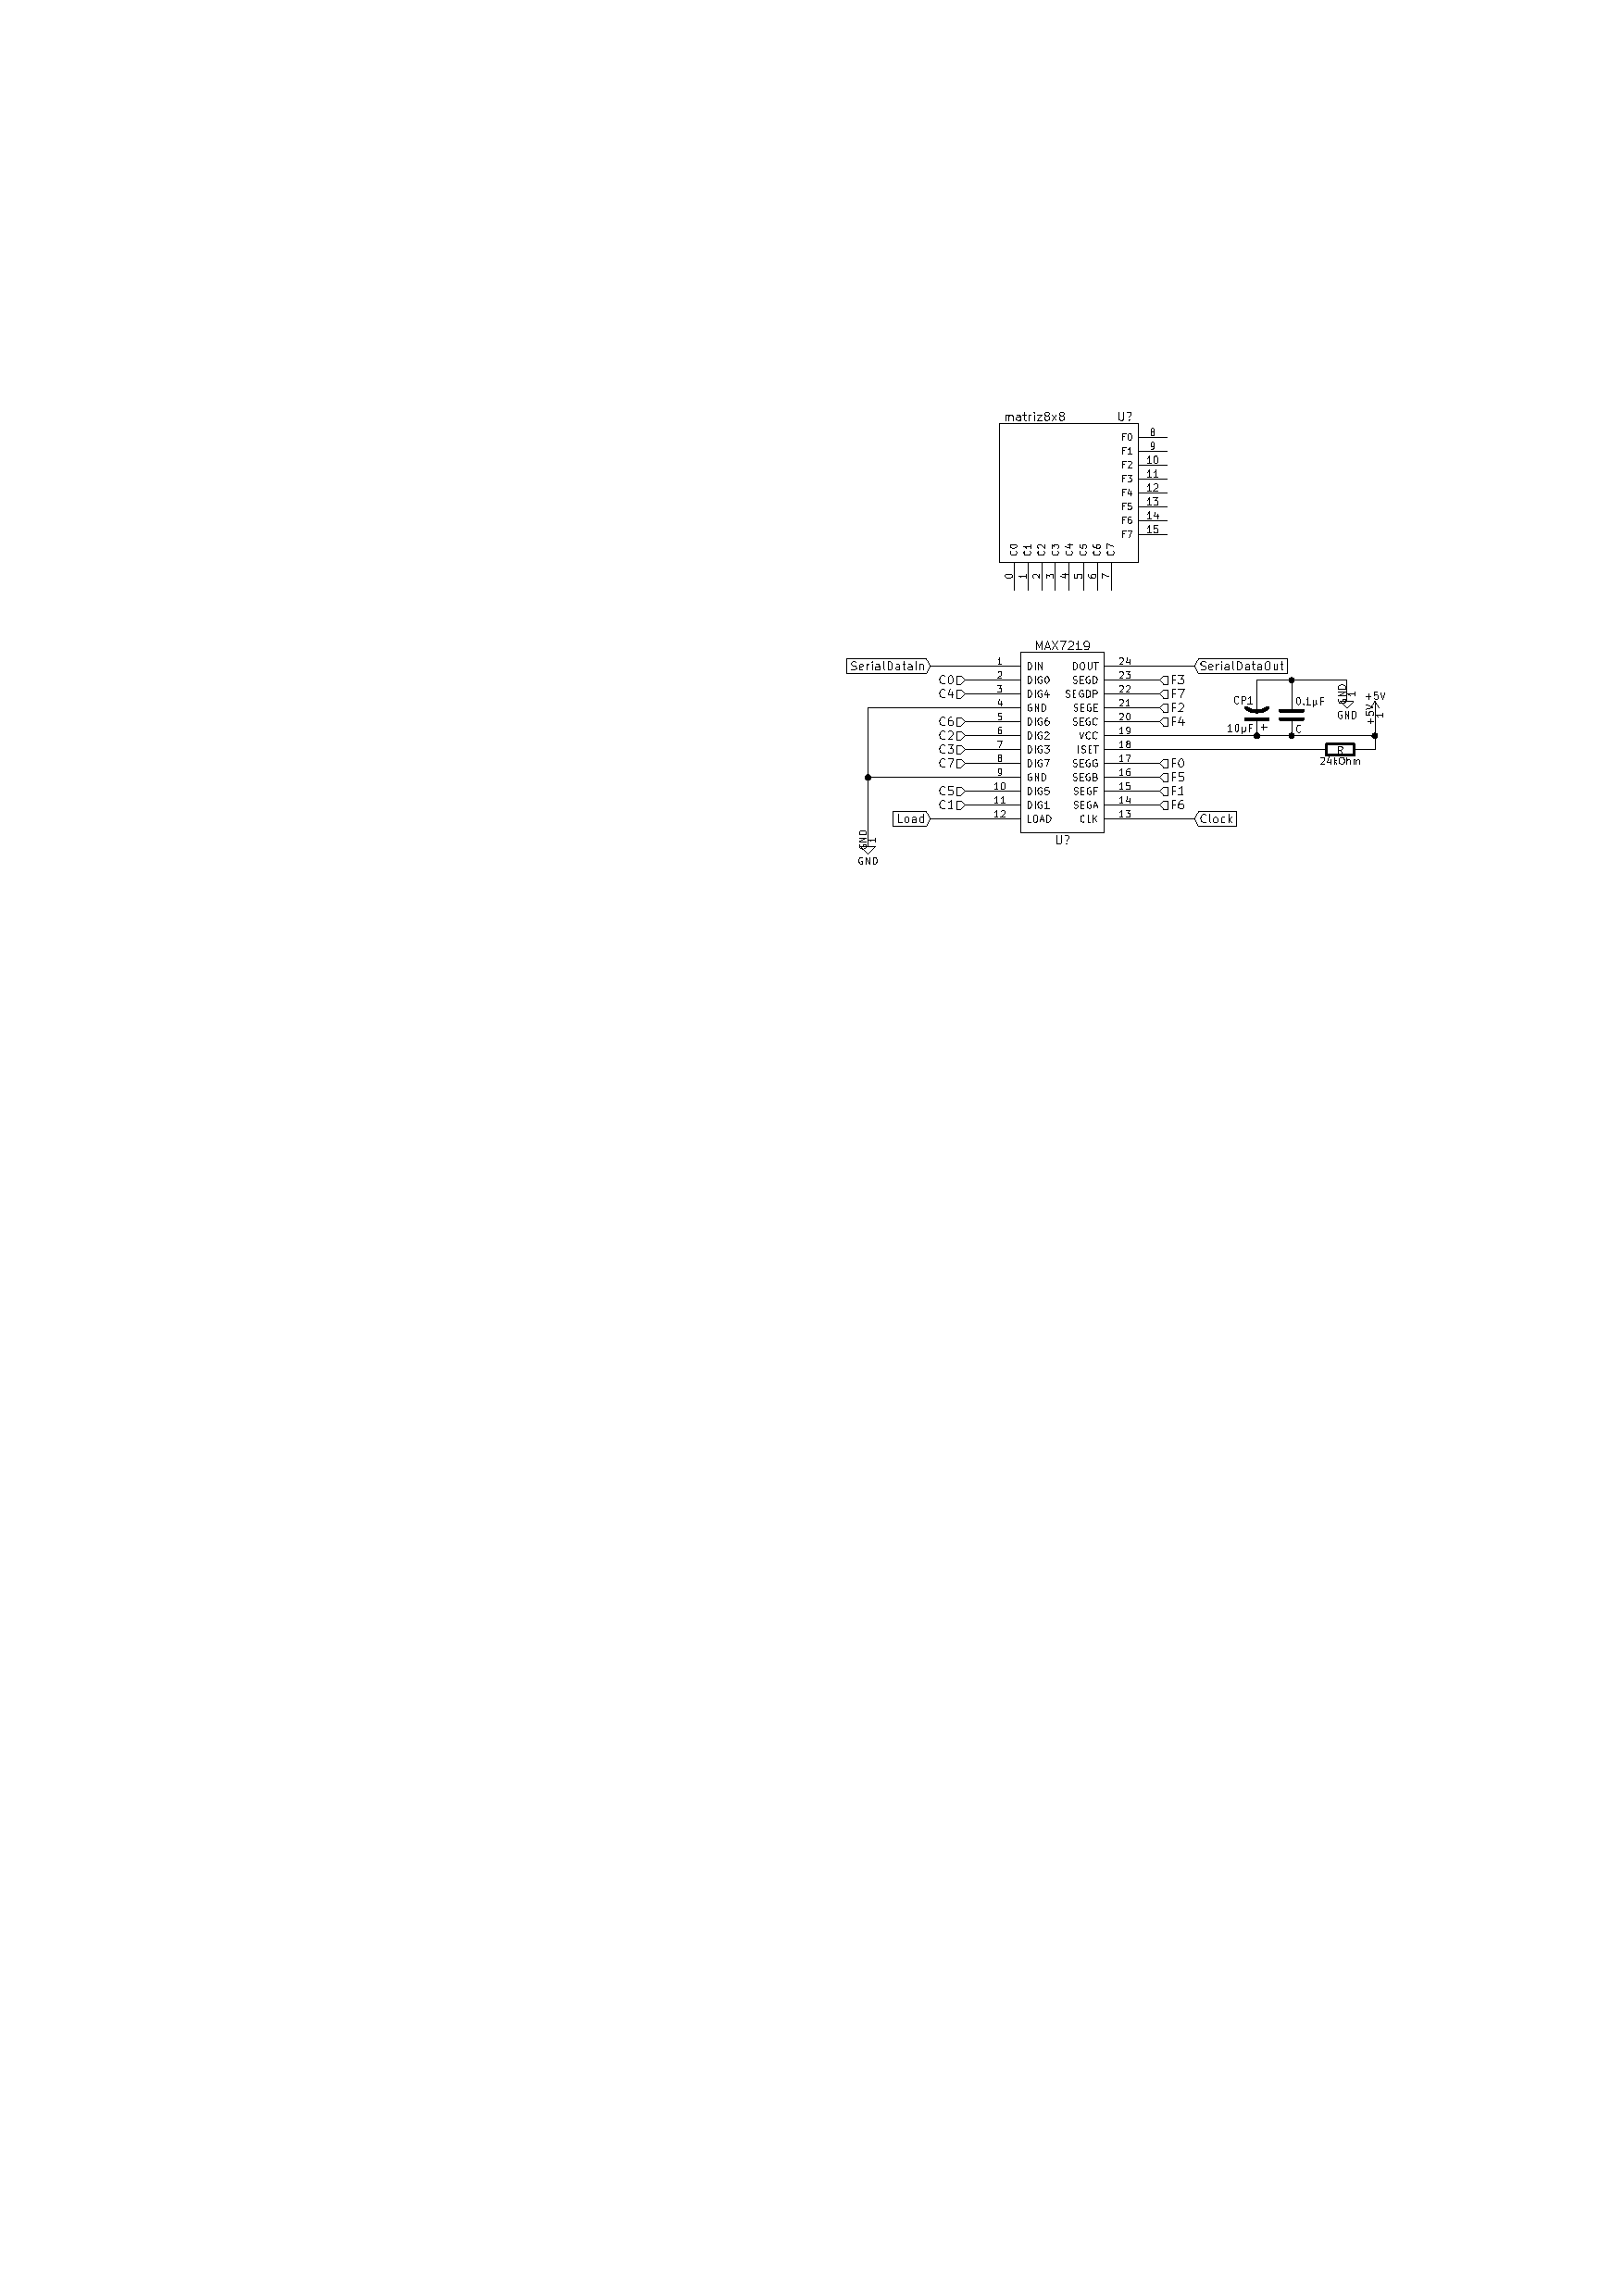
\includegraphics[width=0.8\textwidth]{imagenes/hw/conexion-MAX-matriz.pdf}
	\caption{Conexión entre MAX7219 y su módulo de LEDs.}
	\label{fig:MAX-matriz}
\end{center}
\end{figure}

\begin{figure}[htp!]
\centering
\begin{center}
	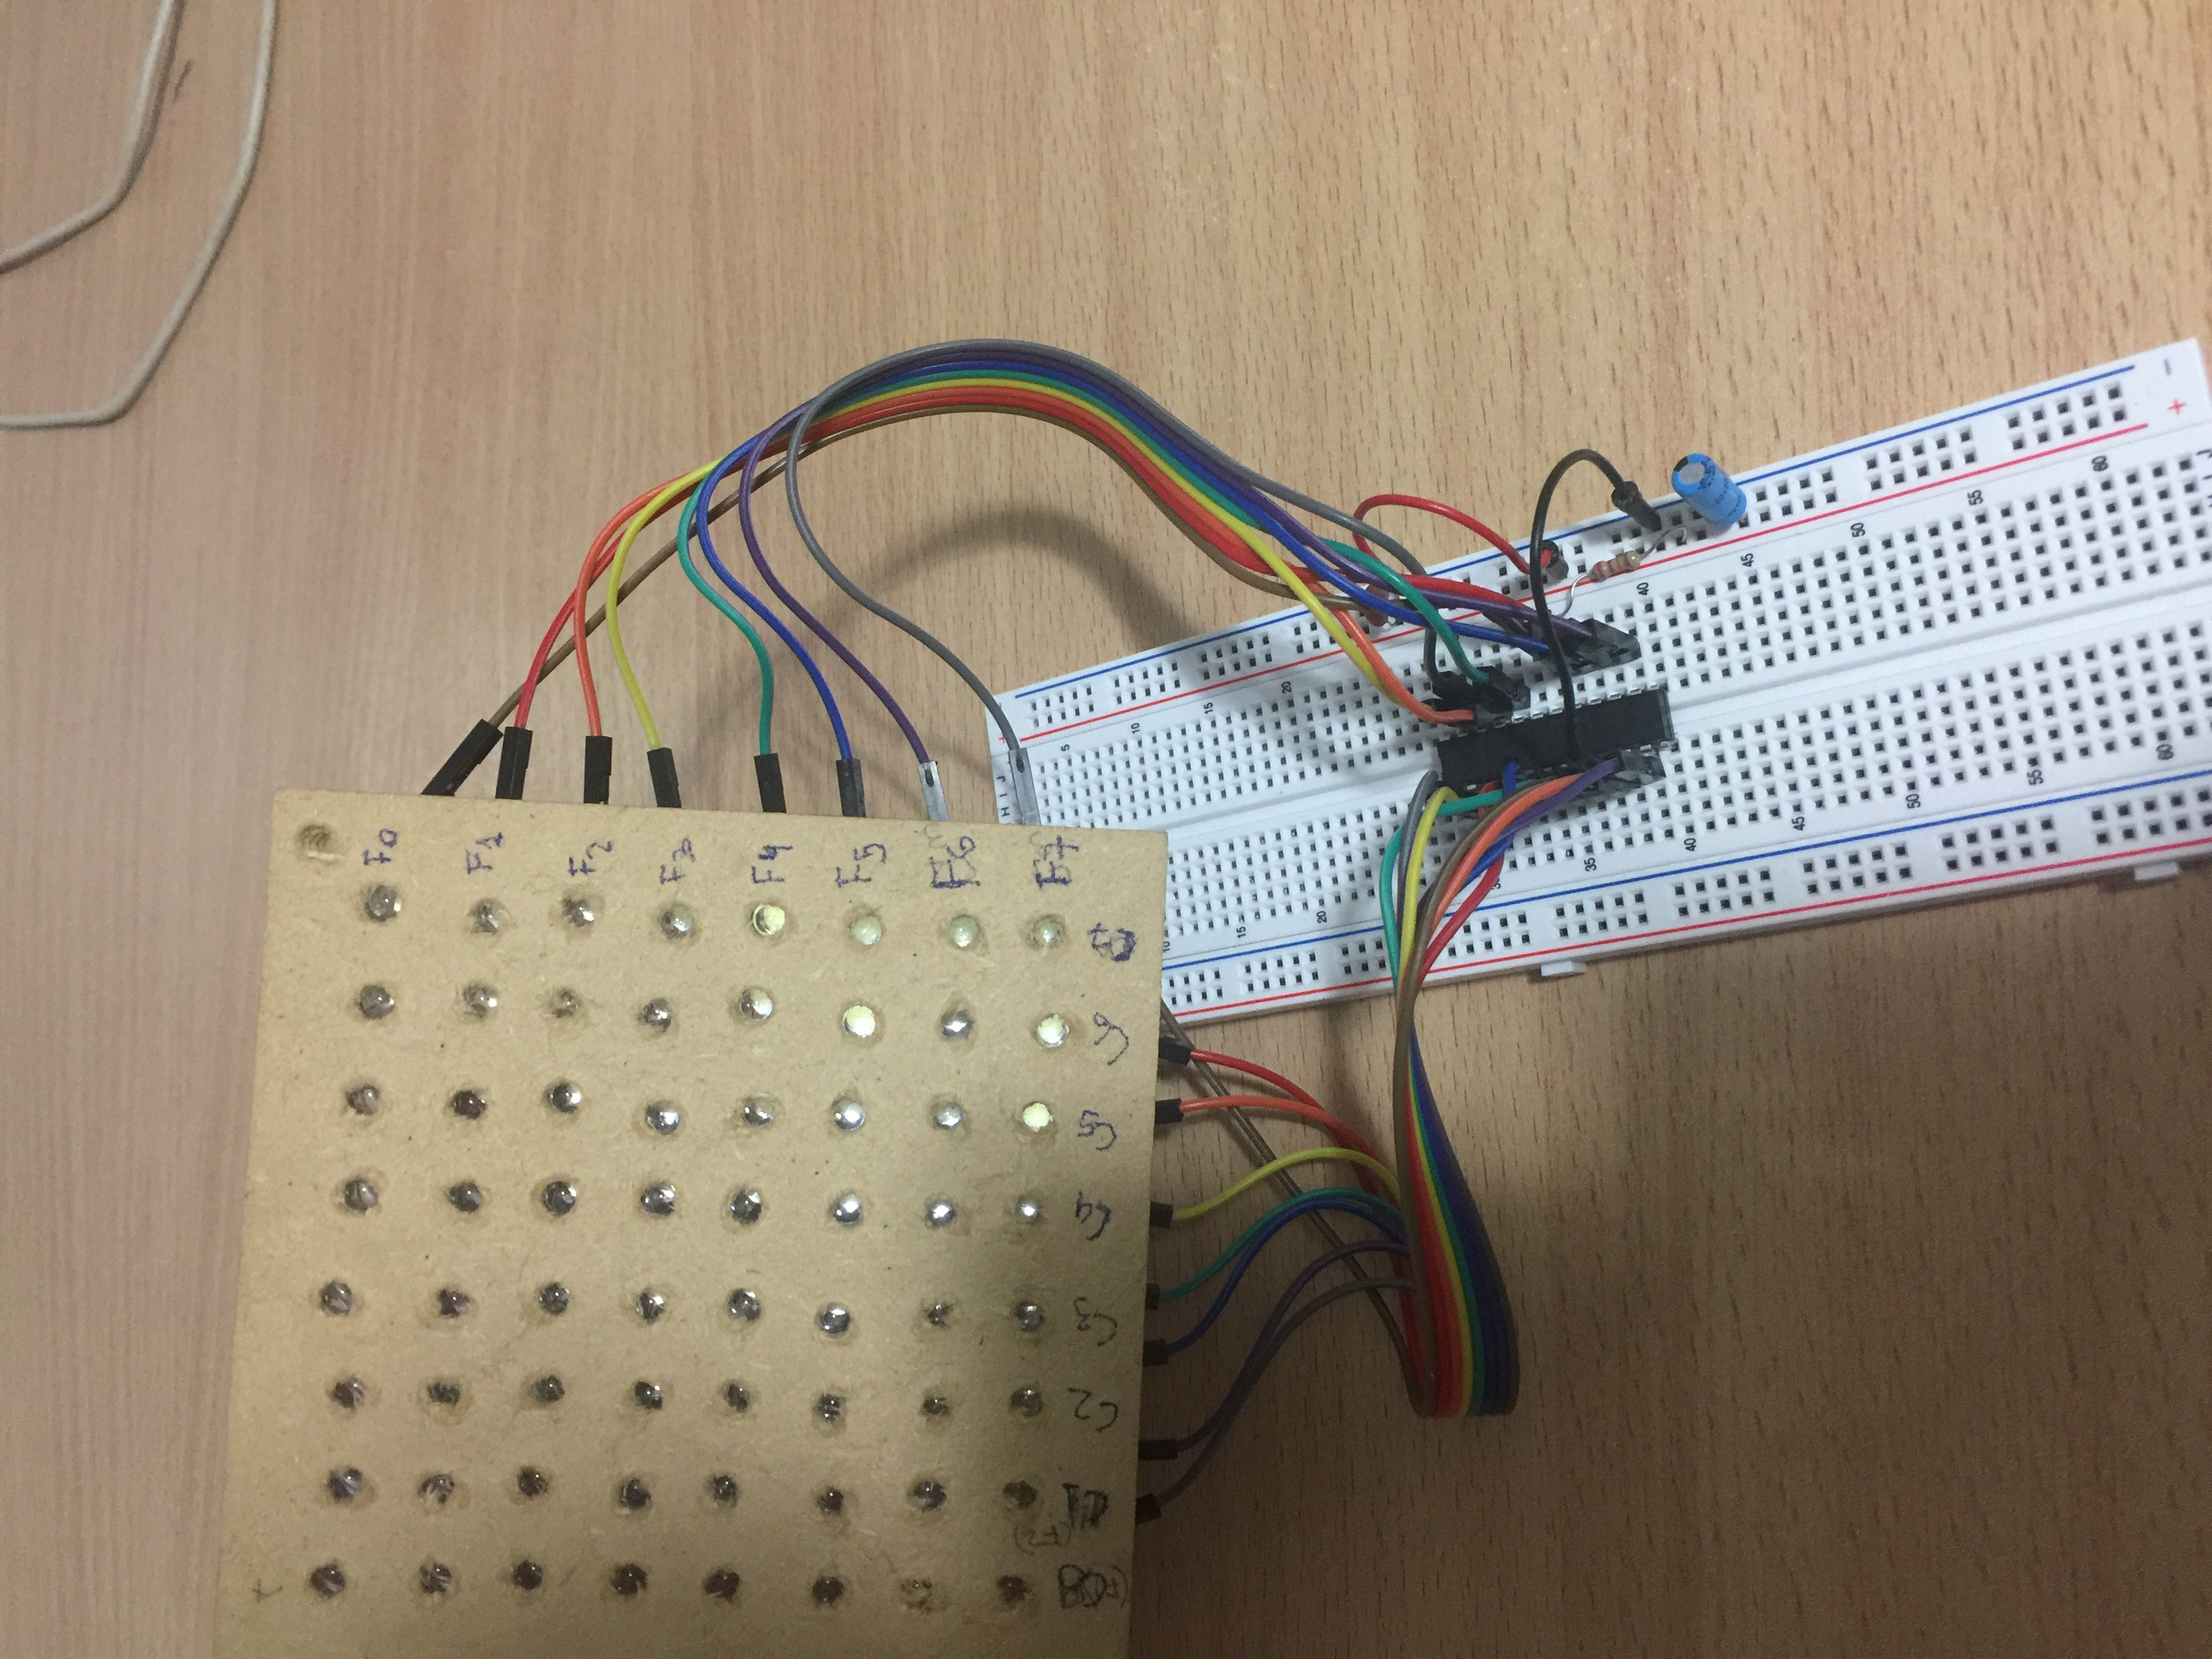
\includegraphics[width=0.7\textwidth]{imagenes/hw/conexion-MAX-matriz.JPG}
	\caption{Fotografía de conexión entre MAX7219 y su módulo de LEDs.}
	\label{fig:MAX-matriz-real}
\end{center}
\end{figure}


\subsection{Matriz de LEDs}
La matriz posee 64 LEDs organizados en ocho filas y ocho columnas, con cátodo común en las columnas como se observa en la figura \ref{fig:modulo-led}. Se analizaron las dimensiones más apropiadas para la utilidad del cartel y se llegó a una separación de 12mm entre LEDs la cual mantiene un dpi apropiado (consiguiendo verse las letras a 10 metros), las demás medidas de pueden observar en la figura \ref{fig:modulo-led-dimensiones}.

Cada uno de los MAX7219 está conectado a una matriz, sus conexiones se pueden observar en el diagrama \ref{fig:MAX-matriz}. Adicionalmente, en la figura \ref{fig:MAX-matriz-real} se observa el prototipo que complementa el esquema de conexión de la figura previamente mencionada.


A la hora de efectuar las conexiones, se debe prestar principal atención a la orientación de la matriz. En la figura \ref{fig:MAX-matriz-real} se indica claramente cuáles son las filas (y su orden) y cuáles son las columnas. Con dicha información el proceso de conexionado se simplifica.

\begin{figure}[!htp]
	\centering
	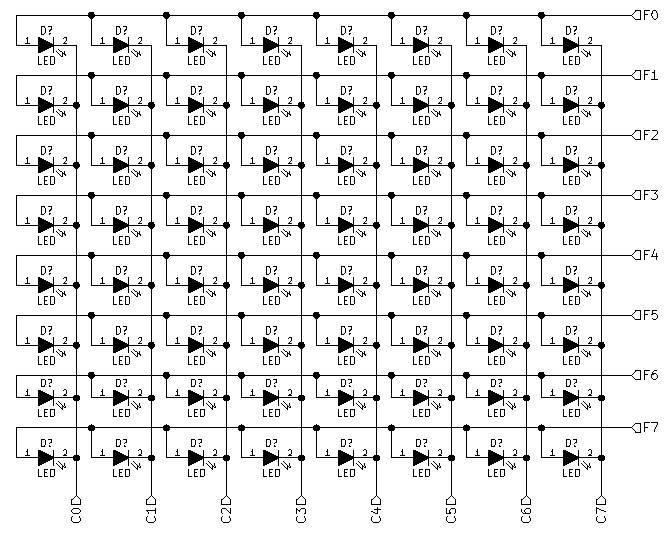
\includegraphics[width=0.7\linewidth]{imagenes/hw/modulo-led.pdf}
	\caption{Esquema de conexiones de la matriz de LEDs.}
	\label{fig:modulo-led}
\end{figure}
\begin{figure}[!htp]
	\centering
	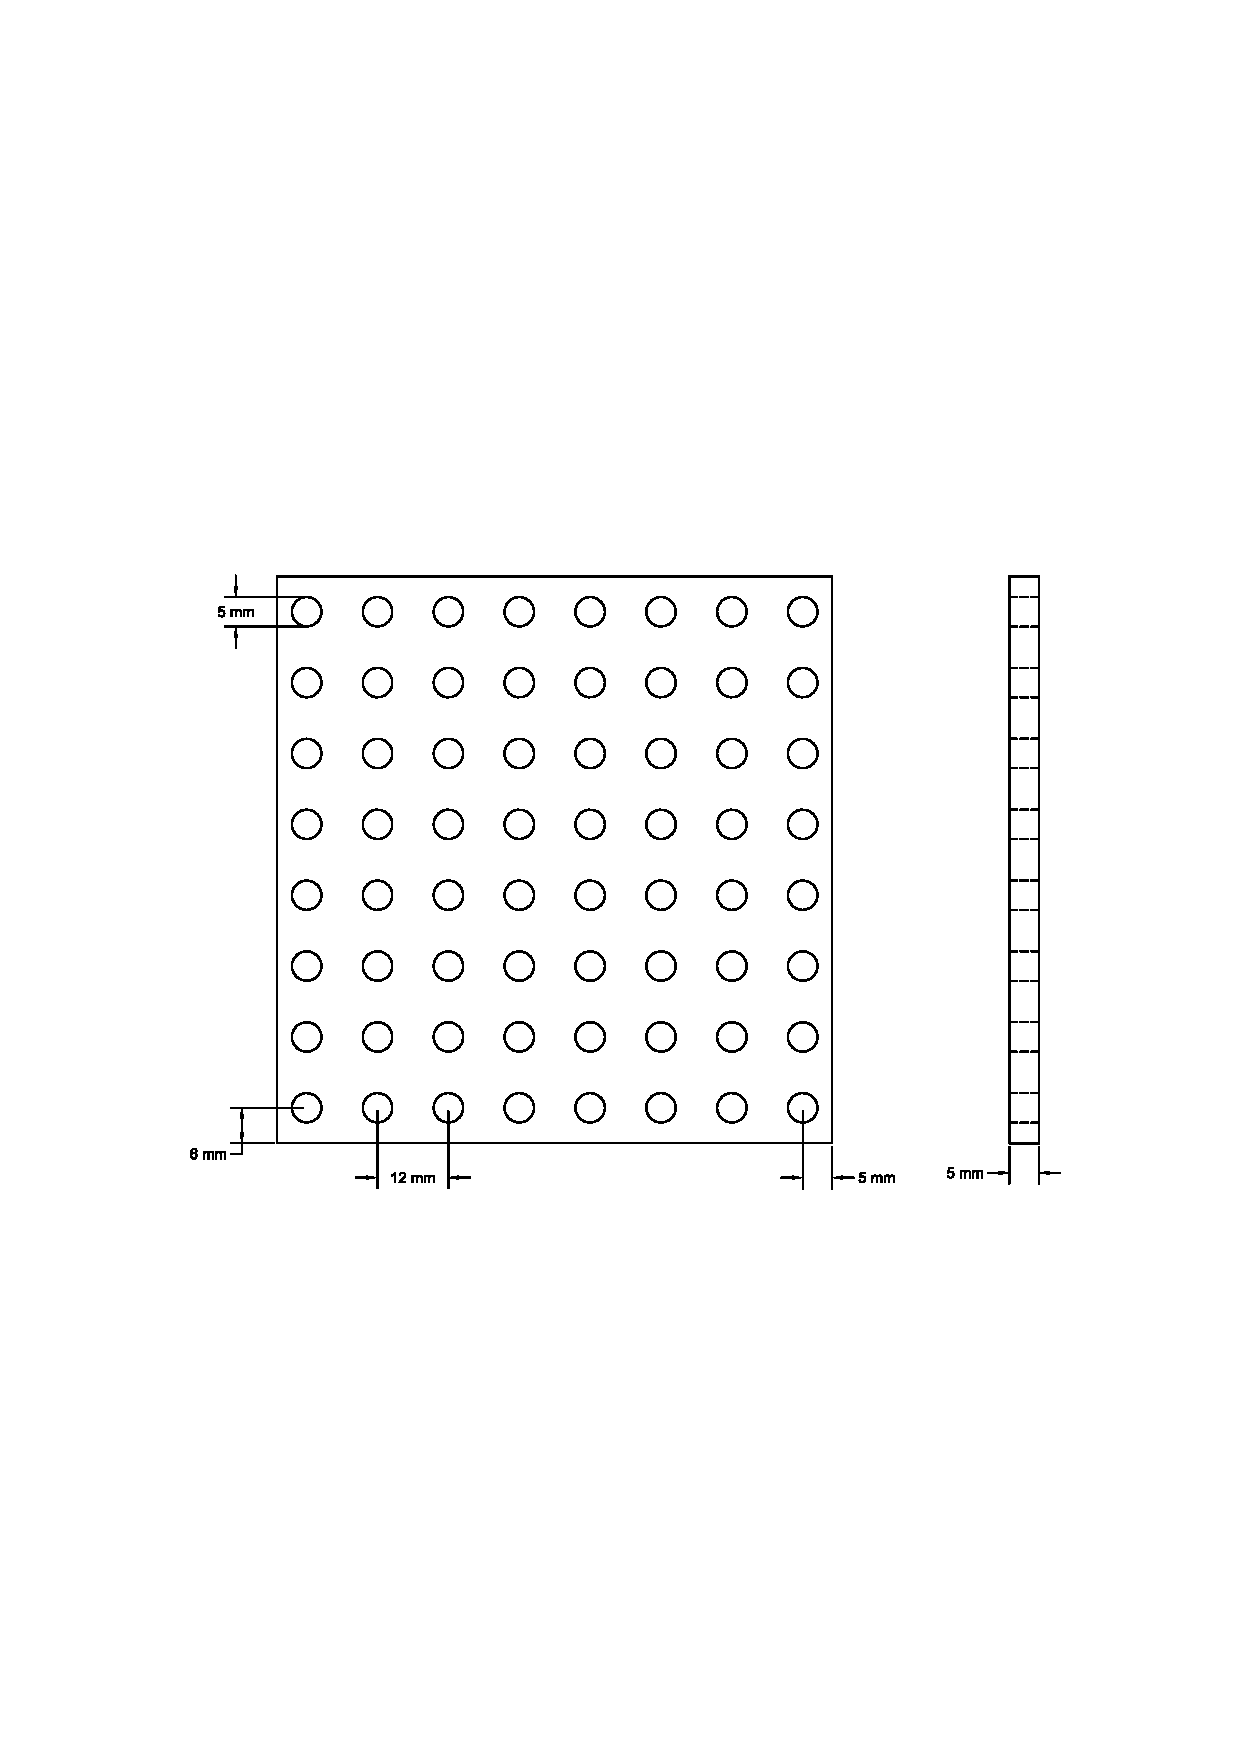
\includegraphics[width=\linewidth]{imagenes/hw/modulo-led-dimensiones.pdf}
	\caption{Dimensiones de la matriz de LEDs.}
	\label{fig:modulo-led-dimensiones}
\end{figure}


\subsection{Comunicación entre los módulos}

\subsubsection{Entre maestro y esclavo}
Como el microcontrolador entrega los datos a 3.3V es necesario convertir estas señales a un voltage que el MAX7219 acepte, la solución que se optó fue incorporar transistores que capaces de transformar 3.3V a 5V. Para ello se conecta tres transistores NPN al circuito, uno por cada señal (DATAIN, LOAD, CLK), se puede observar en la figura \ref{fig:transistors} la conexión.

Los transistores utilizados en el prototipo final son los 2N2369 %(http://www.pci-card.com/2n2369.pdf)
La base es el pin 2, el colector el pin 1 y el emisor el pin 3.
\begin{figure}[ht!]
	\centering
	\begin{center}
		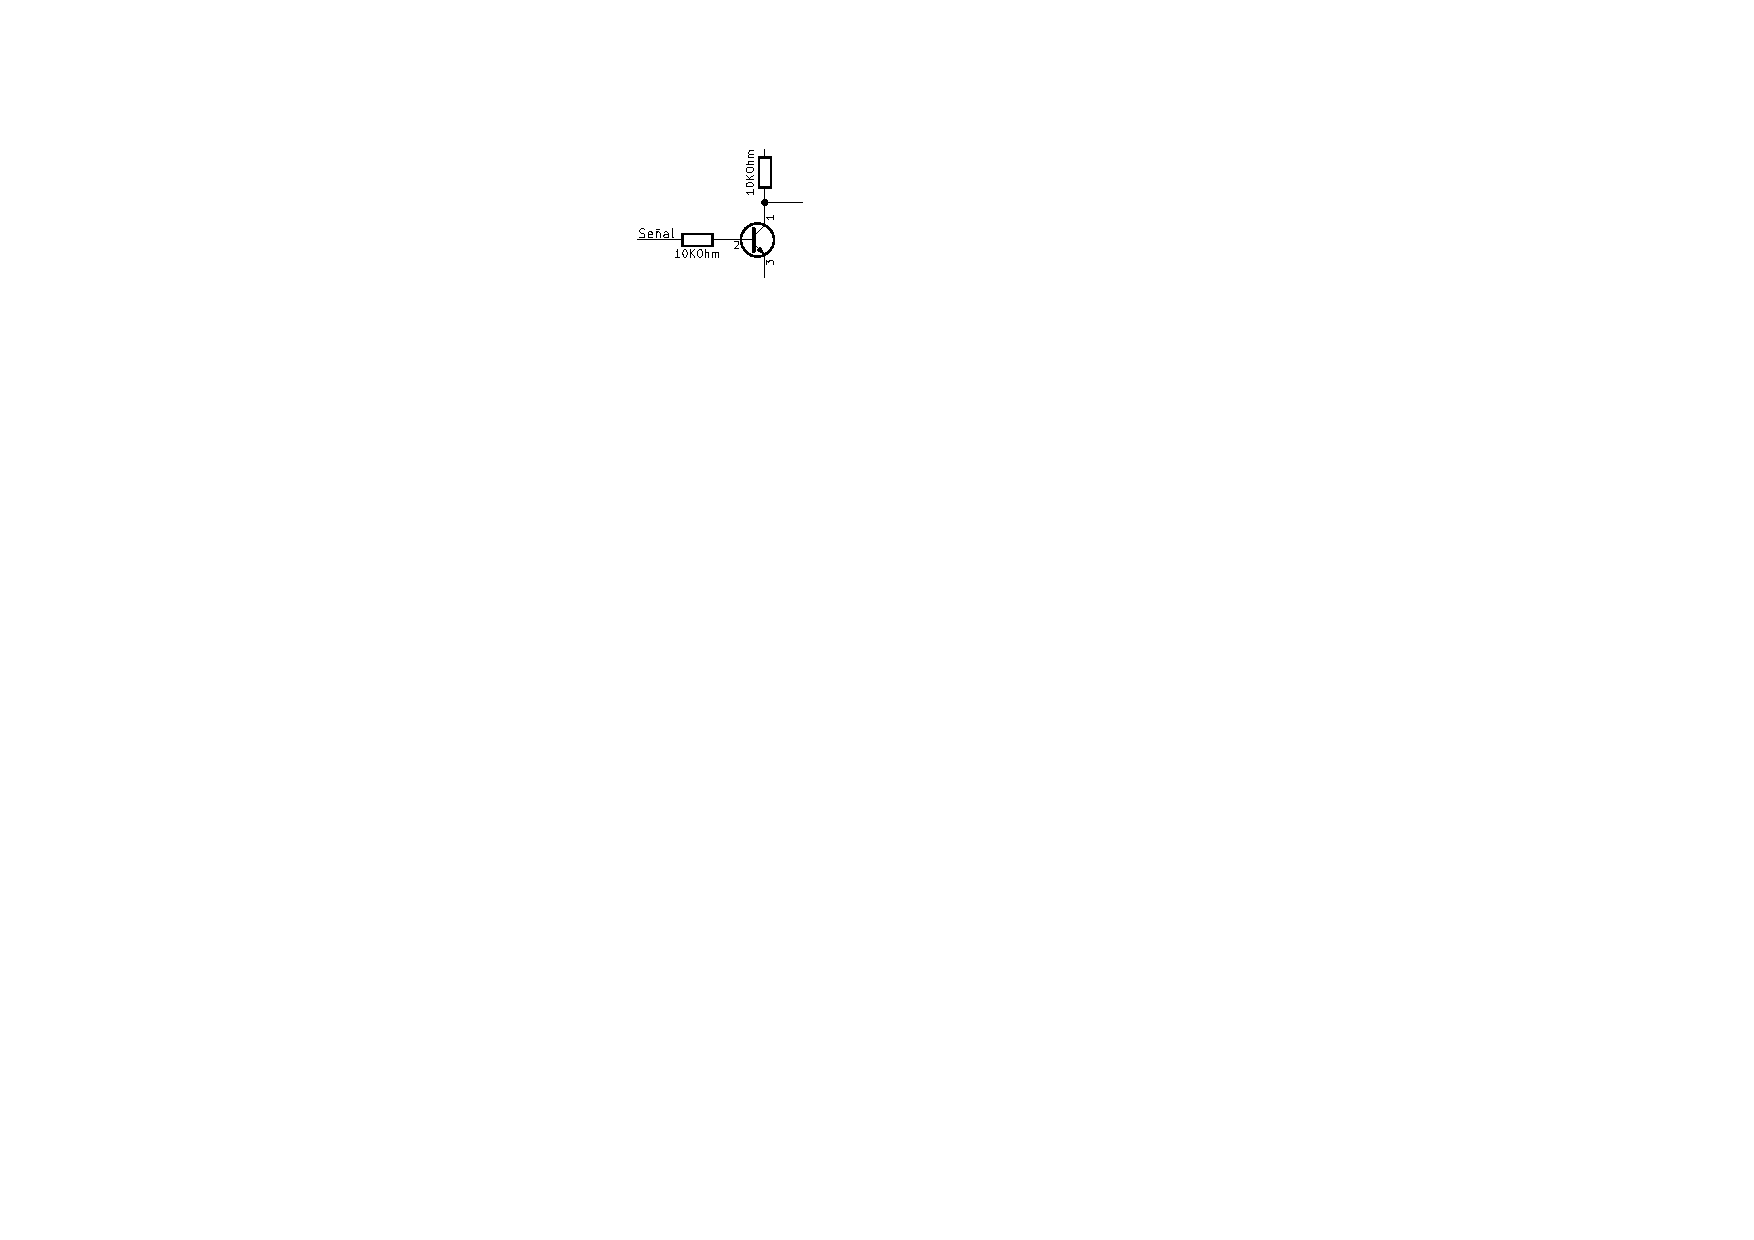
\includegraphics[scale=2]{imagenes/hw/transistor.pdf}
		\caption{Conexión de un transistor, junto con los valores de las resistencias.}
		\label{fig:transistors}
	\end{center}
\end{figure}

\subsubsection{Protocolo de comunicación SPI entre los MAX7219} \label{sec:comunicacion}
Es posible expandir el cartel con N esclavos. En la figura \ref{fig:MAX-MAX} se observa la forma en que se debe realizar la interconexión de los dispositivos integrados.

\begin{figure}[ht!]
	\centering
	\begin{center}
		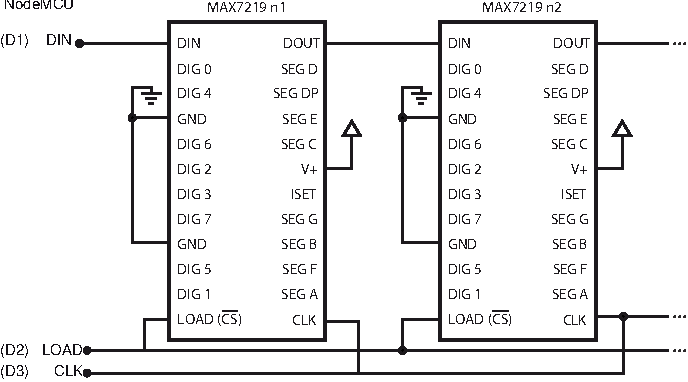
\includegraphics[width=\textwidth]{imagenes/hw/MAX-daisychain.pdf}
		\caption{Conexión entre dos MAX7219.}
		\label{fig:MAX-MAX}
	\end{center}
\end{figure}
Es importante destacar la forma en la que se comunican el microcontrolador con el primer chip shifter, y a su vez, el protocolo que utilizan para comunicarse entre los distintos MAX7219.

La idea general consiste en indicarle a cada chip shifter los leds que debe encender y apagar en cada columna. Para ello debe enviar palabras de dos bytes de manera serial. Es decir, primero envía la información de la columna 1, después la 2, y así siguiendo hasta la 8. El protocolo utilizado es SPI y corresponde a la trama previamente detallada (ver figura \ref{table:trama-spi}).

\begin{table}[ht]
	\centering
	\caption{Trama SPI y su significado.}
	\label{table:trama-spi}
	\begin{adjustbox}{max width=\textwidth}
	\begin{tabular}{|c|c|c|c|c|c|c|c|c|c|c|c|c|c|c|c|}
	\hline
	D15 & D14 & D13 & D12 & D11   & D10   & D9   & D8   & D7 & D6 & D5 & D4 & D3 & D2 & D1 & D0 \\ \hline
	X   & X   & X   & X   & \multicolumn{4}{c|}{ADDRESS} & \multicolumn{1}{c}{ MSB } & \multicolumn{6}{c}{ DATA } & \multicolumn{1}{c|}{ LSB } \\ \hline
	\end{tabular}
	\end{adjustbox}
\end{table}

Para realizar este proceso, la figura \ref{fig:spi-timing-diagram} muestra un diagrama a lo largo del tiempo de la forma de enviar cada bit. En ella se puede observar que el primer paso consiste en bajar la señal de LOAD y esperar un instánte de tiempo (aproximadamente un microsegundo). Luego se debe generar una señal de CLCK de onda cuadrada y de frecuencia de 1Mhz con la mitad de ciclo de trabajo.

El pin conectado al DATAIN del micro, se utiliza para enviar los datos, empezando por el bit más significativo primero. Los datos van a ser leídos por los MAX7219 en el flanco ascendente del CLOCK. Cuando finaliza el envío de los 16 bits, se debe subir la señal de LOAD. En ese momento, el MAX2719 almacena, en sus registros internos, el comando recibido. Todos los comandos son de dos bytes, sin embargo, se puede enviar más de esa cantidad. Esta funcionalidad se utiliza para enviar instrucciones a los demás MAX7219 que están conectados en serie. Lo que ocurre es que la información se recibe en el flanco ascendente de CLK y se envía, hacia el siguiente chip, por el pin DATAOUT en el flanco descendente. De esta forma, en una iteración se pueden configurar una columna de cada módulo de 8x8 LEDs.

\begin{figure}[ht!]
	\centering
	\begin{center}
		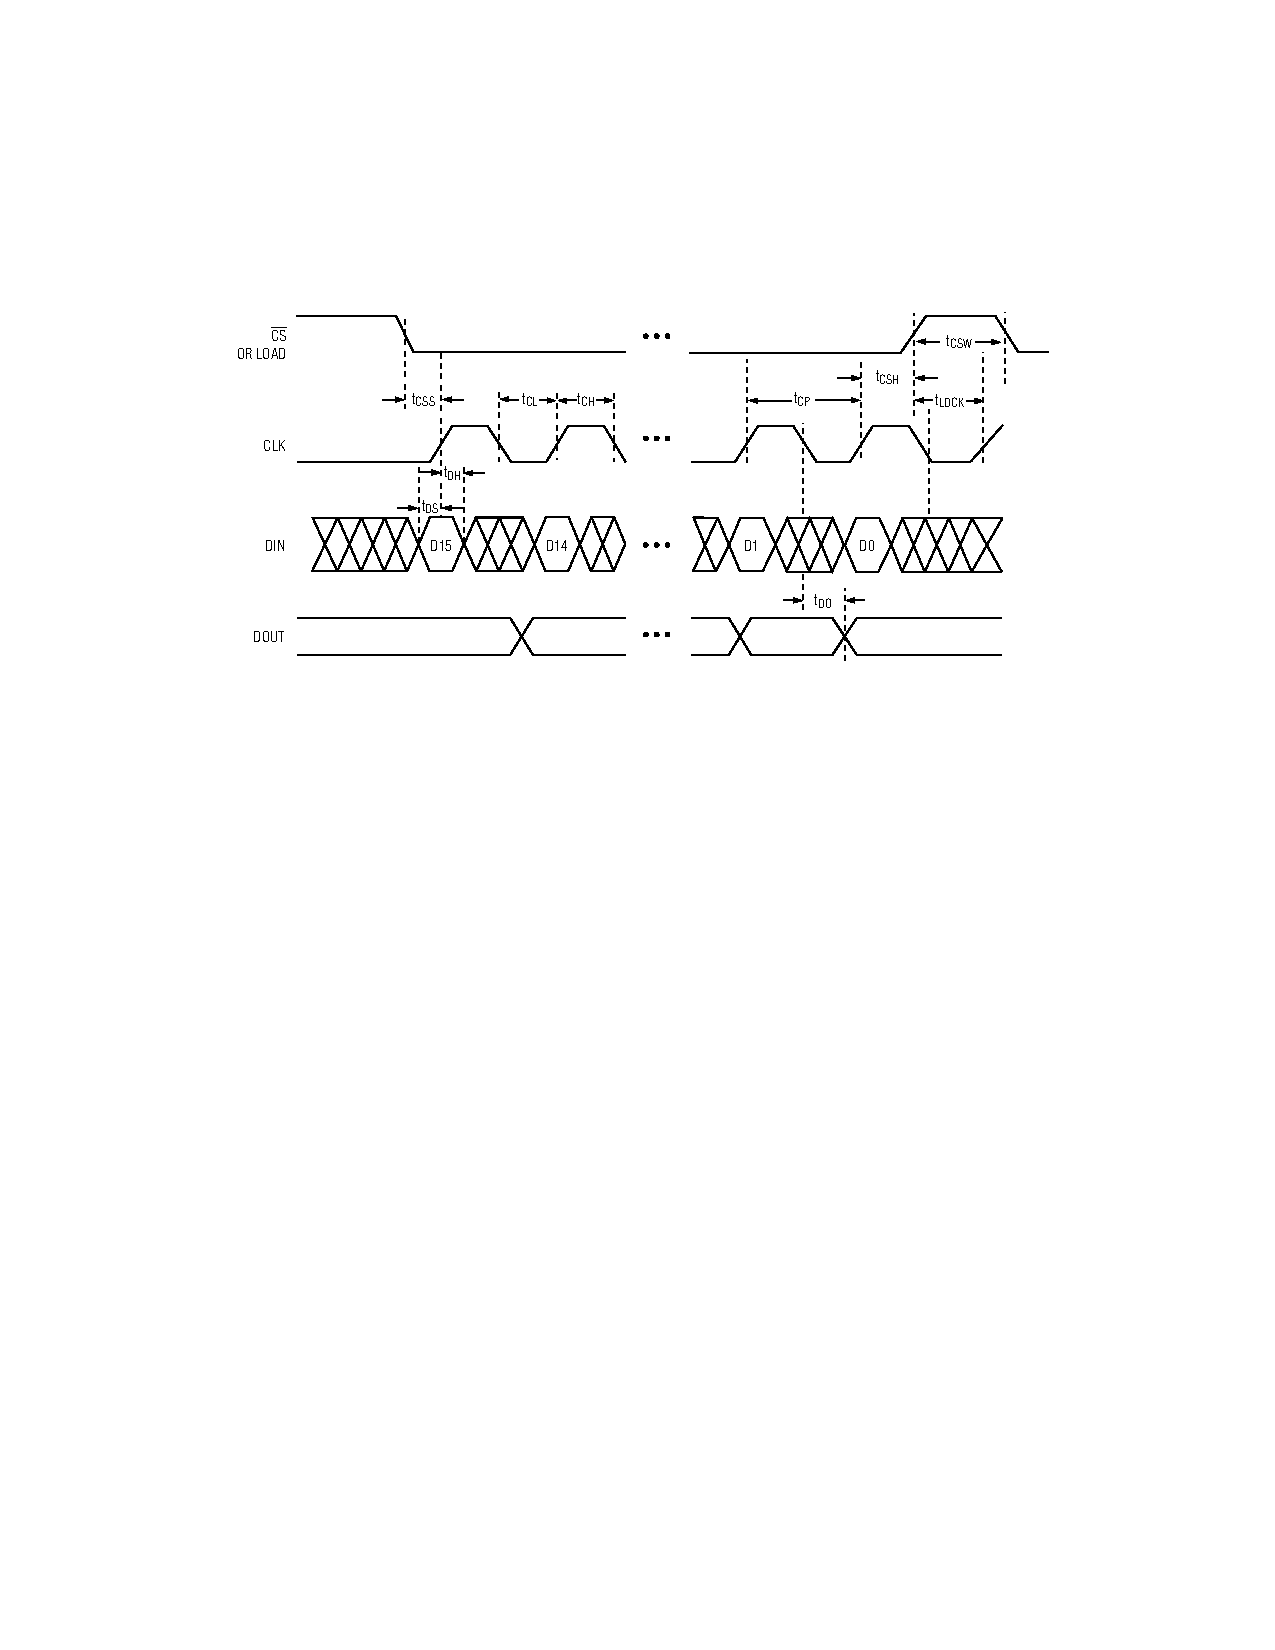
\includegraphics[width=\textwidth]{imagenes/hw/timingDiagram.pdf}
		\caption{Diagrama de tiempo de las señales del MAX7219.}
		\label{fig:spi-timing-diagram}
	\end{center}
\end{figure}
